% Template:     Informe LaTeX
% Documento:    Archivo de ejemplo
% Versión:      8.3.6 (23/08/2024)
% Codificación: UTF-8
%
% Autor: Pablo Pizarro R.
%        pablo@ppizarror.com
%
% Manual template: [https://latex.ppizarror.com/informe]
% Licencia MIT:    [https://opensource.org/licenses/MIT]

% ------------------------------------------------------------------------------
% NUEVA SECCIÓN
% ------------------------------------------------------------------------------
% Las secciones se inician con \section, si se quiere una sección sin número se
% pueden usar las funciones \sectionanum (sección sin número) o la función
% \sectionanumnoi para crear el mismo título sin numerar y sin aparecer en el índice
\section{Preguntas de desarrollo}
\begin{enumerate}
	\item \textbf{Describa el comportamiento de un fotón y sus propiedades (liste al menos 7
	características relevantes) y Determine la Energía de un Fotón para $\lambda =1550nm$ usada para una Comunicación Óptica y compárela con la Energía de un Fotón para $\lambda =10^{-2}m$ en Comunicación por Microondas. ¿Qué podría deducir de esto?}
Dado que se busca describir el comportamiento de un foton y sus propiedades, las cuales vienen dadas por:
\begin{itemize}
	\item La energia esta cuantizada, eso significa que ser absorvida o emitida en paquetes discretos. Se relaciona mediante la formula:
	\begin{align}
		E = h \cdot f
	\end{align}
	donde h es la constante de Planck y f es la frecuencia de la onda.
	\item No presenta una masa en reposo, lo que le permite viajar a la velocidad de la luz.Esto viene de la teoria de la relatividad de Einstein que establece que cualquier particula sn masa debe viajar a la velocidad de la luz.
	\item Los fotones presentan un comportamiento dual, actuando tanto como particula y como onda. Esto se puede observar en el experimento de la doble rendija.
	\item A pesar de que los fotones no tienen masa, si poseen momento lineal, el cual se puede calcular mediante la formula:
	\begin{align}
		p = \frac{E}{c}
	\end{align}
	Y por tanto pueden ejercir presion sobre un objeto.
	\item Los fotones no poseen carga electrica, lo que les permite viajar a traves de un campo electrico sin ser afectados o magneticos
	\item Los fotones presentan el principio de incertidumbre de Heisenberg, lo que significa que no se puede conocer la frecuencia y la posicion de un foton al mismo tiempo.
	\item Los fotones presentan polarizacion , que es la propiedad asocada a la orientacion de una onda electromagnetica, existen diferentes tipos de esta como la polarizacion lineal, circular y eliptica,etc.
\end{itemize}
Por otro lado se busca el obtener la energia del foton para una longitud de onda de 1550nm y $10^{-2}m$, para ello se puede utilizar la formula (1) y se obtiene que:
\begin{align}
	E_{1550nm} = \frac{6.26 \cdot 10^{-34} [J] \cdot 3 \cdot 10^{8}[\frac{m}{s}]}{1.55\cdot 10^{-6}m} = 1.28 \cdot 10^{-19} J
\end{align}
Luego para la longitud de onda de $10^{-2}m$ se obtiene que:
\begin{align}
	E_{10^{-2}m} = \frac{6.26 \cdot 10^{-34} [J] \cdot 3 \cdot 10^{8}[\frac{m}{s}]}{10^{-2}m} = 1.99 \cdot 10^{-23} J
\end{align}
Dado que se esta realizando una comparacion de energia entre la energia para diferentes longitudes de onda y aplicaciones en la industria (Optica y microondas). Se puede concluir que los fotones opticos tendran mucho mas energia que los fotones de microondas y por tanto permite que se puedan transmitir mas informacion.
\item \textbf{Explique los siguientes fenómenos de comportamiento de la Luz: Reflexión,
Refracción, Interferencia, Difracción, Dispersión y Polarización.}
Se busca el explicar los siguientes fenomenos de la luz, por lo tanto tenemos que:
\begin{itemize}
	\item \textbf{Reflexión:} Es el fenomeno en el cual la luz cambia de medio y se refleja en la superficie de un material. Esto se puede explicar mediante la ley de reflexion que establece que el angulo de incidencia es igual al angulo de reflexion ($\theta_{r} = \theta_{i}$). Es importante destacar que la reflexion puede ser especular o difusa, dependiendo de la superficie y ademas se puede producir una reflexion total interna si el angulo de incidencia es mayor al angulo critico.\\\\
	La reflexión interna total es la la idea principal de como funciona la fibra optica , esta ocurre dentro de la fibra óptica. Cuando la luz se introduce en el núcleo de la fibra óptica, debido a la diferencia de índice de refracción entre el núcleo y el revestimiento, la luz se refleja repetidamente dentro del núcleo, manteniéndose confinada en la fibra y permitiendo la transmisión de datos a largas distancias.
	\item \textbf{Refracción}:Es el fenomeno en el cual la luz cambia de medio y se desvia de su trayectoria original.Esto se debe a la diferencia de velocidad de la luz en los distintos medios y se puede explicar mediante la ley de Snell que establece que el producto del indice de refraccion del medio 1 y el seno del angulo de incidencia es igual al producto del indice de refraccion del medio 2 y el seno del angulo de refraccion. Es importante destacar que la refraccion puede ser positiva o negativa dependiendo del indice de refraccion del medio.\\\\
	La refracción ocurre cuando la luz entra en la fibra óptica desde el aire o desde un conector. La luz cambia su dirección al pasar de un medio con un índice de refracción (como el aire) a otro con un índice de refracción diferente (como el núcleo de la fibra óptica).
	\item \textbf{Interferencia:} Es el fenomeno en el cual dos ondas se superponen y se combinan para formar una onda resultante. Esto se puede explicar mediante el principio de superposicion que establece que la amplitud de la onda resultante es la suma de las amplitudes de las ondas que se superponen. Es importante destacar que la interferencia puede ser constructiva o destructiva dependiendo de la diferencia de fase entre las ondas.\\\\
	La interferencia puede ocurrir en sistemas de multiplexación por división de longitud de onda (WDM), donde diferentes señales de luz con diferentes longitudes de onda viajan por la misma fibra. Si estas señales no están bien aisladas, pueden interferir entre sí, causando pérdida de calidad o distorsión de la señal.

	\item \textbf{Difracción:} Es el fenomeno en el cual la luz se desvia alrededor de un obstaculo o pasa por una rendija. Esto se puede explicar mediante el principio de Huygens que establece que cada punto de un frente de onda se comporta como una fuente de ondas secundarias. Es importante destacar que la difraccion es mas pronunciada si la longitud de onda de la luz es del mismo orden de magnitud que el obstaculo o la rendija.\\\\
	Si la fibra tiene una curvatura o una imperfección, la luz se difractará alrededor de estas imperfecciones, lo que puede causar pérdida de señal o distorsión de la señal.
	
	\item \textbf{Polarización:} Es la orientación de las oscilaciones del campo eléctrico de una onda de luz. La luz natural no polarizada tiene oscilaciones en todas las direcciones perpendiculares a su dirección de propagación, mientras que la luz polarizada oscila en una única dirección. La intensidad de la luz polarizada despues de pasar por un polarizador se describe por la ley de Malus.\\\\
	La polarización es importante en la fibra óptica, ya que la luz polarizada puede ser transmitida a través de la fibra de manera más eficiente que la luz no polarizada. La luz polarizada también se utiliza en aplicaciones de comunicación óptica para transmitir información a través de la luz.
\end{itemize}
Posterior a la explicacion de los fenomenos de la luz, se puede concluir que estos fenomenos son fundamentales en la transmision de informacion mediante la luz y son la base de la fibra optica y la comunicacion optica. Para el caso particular del pryecto ELT que permitira la observacion de objetos en el espacio, se utilizara transmision de grandes cantidades de volume de datos desde un Datacenter, y la presicion de la transmision de datos es crucial.En base a la informacion proporcionada, se puede concluir que una buena opciones es utilizar fibras PM (Polarization Maintaining), algunos de estos motivos son:
\begin{itemize}
	\item Este tipo de fibras puede ser usada den largas distancias, donde uno de los problemas principales es la PDF (Polarization Dependent Loss) que puede afectar la calidad de la señal,ya que los diferentes modos de polarización se propagan a distintas velocidades. Las fibras PM están diseñadas para mantener la polarización a lo largo de la fibra, lo que ayuda a minimizar la dispersión y la distorsión.
\end{itemize}
Es por esto, que se recomienda el utilizar este tipo de fibra.
\item \textbf{Le solicitan que usted recomiende la Potencia óptica del transmisor para la
cuál la Potencia de salida sea el valor promedio de la Sensibilidad óptica y la
Potencia de saturación. Por otro lado, le solicitan calcular el número de fotones
emitidos por hora de acuerdo a la Potencia recomendada de la fuente.}
\begin{figure}
	\centering
	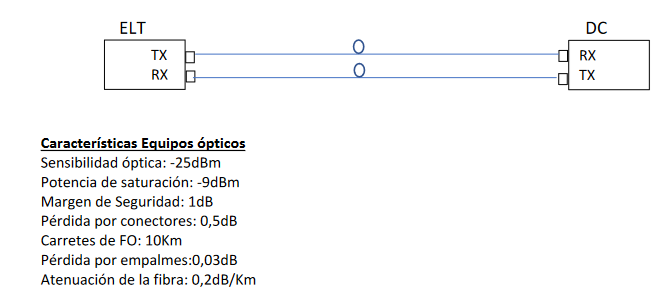
\includegraphics[width=0.8\linewidth]{img/P3_1.png}
	\caption{Esquema planteado}
	\label{fig:imagen1}
\end{figure}
Dado el esquema anterior, luego se busca que la potencia optica del transmisor sea el promedio de la sensibilidad optica y la potencia de saturacion, por lo tanto se tiene que:
\begin{align}
	P_{salida} &= \frac{P_{\text{Sensibilidad optica}} + P_{\text{Potencia de saturacion }}}{2}
	&= \frac{-25+ (-9)}{2} = -17 [dBm]
\end{align}
Por lo que la potencia recomendada del transmisor debera ser de -17 dBm. Luego se busca calcular el numero de fotones emitidos por hora. Para esto se pasa a Watts la potencia recomendada,dado que se encuentra en dBm
\begin{align}
	P_{recomendada} &= 10^{-17/10} = 0.02 [mW]
	&= 0.02 \cdot 10^{-3} = 2 \cdot 10^{-5} [W]
\end{align}
De esta manera se obtiene la potencia en Watts, luego se busca calcular el numero de fotones emitidos por hora, para ello se calcula la energia de un foton a la longitud de operacion:
\begin{align}
	E_{foton} &= \frac{6.26 \cdot 10^{-34} [J] \cdot 3 \cdot 10^{8}[\frac{m}{s}]}{1.55\cdot 10^{-6}m} = 1.28 \cdot 10^{-19} J
\end{align}
Luego sabemos que la potencia es la energia por unidad de tiempo, por lo que se tiene que:
\begin{align}
	P = \frac{E}{t} \Rightarrow E = P \cdot t
\end{align}
Con lo que se tiene que el numero de fotones emitido por segundo es:
\begin{align}
	N_{fotones} &= \frac{P}{E_{foton}} = \frac{2 \cdot 10^{-5} [W]}{1.28 \cdot 10^{-19} [J]} = 1.56 \cdot 10^{14} [fotones/s]
\end{align}
Luego se busca calcular el numero de fotones emitidos por hora, para ello se tiene que:
\begin{align}
	N_{fotones/h} &= N_{fotones/s} \cdot 3600 = 1.56 \cdot 10^{14} \cdot 3600 = 5.62 \cdot 10^{17} [fotones/h]
\end{align}
Con lo que se obtiene la cantidad de fotones por hora emitidas para la potencia reocmendada.
\item \textbf{Para la fibra monomodo proyectada se tiene un índice de refracción del núcleo $n_1 = 1.5$ e índice de refracción del manto o revestimiento (\textit{cladding}) $n_2 = 1.48$ por el cual se produce la reflexión interna total al interior de la fibra. Calcule el ángulo de apertura de la fibra que forma el cono de aceptación para el cual los rayos de luz que vienen de la fuente entran a la fibra. (Con este ángulo se calcula la Apertura Numérica (NA) que le servirá al cliente para la compra de la fuente óptica). Investigue y calcule el NA y luego el número V.}
Dado que se busca obtener el angulo de apertura de la fibra, primero se obtendra la apertura numerica la cual viene dada por:
\begin{align}
	NA = \sqrt{n_{1}^{2} - n_{2}^{2}}
\end{align}
Dado los valores de indice de refraccion del enunciado, luego tenemos que:
\begin{align}
	NA = \sqrt{1.5^{2} - 1.48^{2}} = 0.244
\end{align}
Con este valor se logra obtener el angulo de aceptacion el cual corresponde a :
\begin{align}
	\theta_{a} = \sin^{-1}(NA) = \sin^{-1}(0.244) = 14.1^{\circ}
\end{align}
Luego se busca obtener el numero V, el cual se denomina frecuencia normalizada, el cual es una numero adimensional y determina cuandos modos una fibra puede soportar, se obtiene como:
\begin{align}
	V = \frac{2\pi a NA}{\lambda}
\end{align}
Que para nuestro caso particular un radio de 9 micrometros se obtiene que el numero de modos que aguanta esta fibra optica:
\begin{align}
	V = \frac{2\pi \cdot 9 \cdot 10^{-6} \cdot 0.244}{1.55 \cdot 10^{-6}} = 0.72
\end{align}
\item Los ingenieros e investigadores saben que así como las pérdidas y atenuaciones de los sistemas de fibra óptica afectan las potencias ópticas, las dispersiones afectan a las tasas de transmisión de datos, por lo que les preocupa algo que le han comentado acerca de los efectos de la dispersión por modo de polarización (PMD) para velocidades superiores a 10Gbps y largas distancias.
\begin{itemize}
	\item \textbf{Investigue y explique primero que tipos de dispersión afectan a una fibra
	óptica (dispersión modal, dispersión cromática, dispersión por guía-onda y PMD).}\\\\
	En una fibra optica se tienen multiples tipos de dispersion que puede afectar la transmision de datos y calidad de datos, estos son:
	\begin{itemize}
		\item \textbf{Dispersión modal:} Es la dispersión que se produce debido a la diferencia en la velocidad de propagacion de los distintos modos de propagacion de la luz en la fibra. Esto se debe a que los modos de propagacion se propagan a distintas velocidades y por tanto la luz se dispersa en el tiempo.\\
		\item \textbf{Dispersión cromatica:} Es la dispersion que se produce debido a la diferencia en la velocidad de propagacion de los distintos colores de la luz en la fibra. Esto se debe a que los distintos colores de la luz se propagan a distintas velocidades y por tanto la luz se dispersa en el tiempo.\\
		\item \textbf{Dispersión por guia-onda:} Es la dispersion que se produce debido a la diferencia en la velocidad de propagacion de los distintos modos de polarizacion de la luz en la fibra. Esto se debe a que los modos de polarizacion se propagan a distintas velocidades y por tanto la luz se dispersa en el tiempo.\\
		\item \textbf{PMD:} Es la dispersion que se produce debido a la diferencia en la velocidad de propagacion de los distintos modos de polarizacion de la luz en la fibra. Esto se debe a que los modos de polarizacion se propagan a distintas velocidades y por tanto la luz se dispersa en el tiempo. 
	\end{itemize}
	\item \textbf{Explique de manera sencilla y con un diagrama porqué la birrefringencia del material de la fibra óptica es la causante del PMD, y cuál debería ser el Coeficiente de PMD a solicitar al fabricante de la fibra óptica para L=60Km, 10Gbps y PMD máximo}\\\\
	En base al paper entragado se busca obtener el coeficiente de PMD, PMD maximo para un L=60Km y 10Gbps, para ello se tiene que consierar que el intervalo de tiempo $T_b$ se calcula como:
	\begin{align}
		T_b = \frac{1}{\text{Bit Rate}} = \frac{1}{10 \cdot 10^{9} \text{bits/s}} = 100[ps]
	\end{align}
	De esta manera en base a las formulaciones realizadas en el paper se tiene que el coeficiente de PMD maximo se logra obtener como:
	\begin{align}
	PMD_{max}&=\frac{T_B}{10}\\
	&= \frac{100[ps]}{10} = 10[ps]
	\end{align}
	De esta manera se obtiene el valor de PMD maximo para la fibra optica, con este ultimo es posible obtener el valor de $PMD_{coef}$ como:
	\begin{align}
		PMD = PMD_{coef} \cdot \sqrt{L}
	\end{align}
	Dado que conocemos el valor de $PMD_{max}$ tenemos luego que:
	\begin{align}
		10[ps] = PMD_{coef} \cdot \sqrt{60} \Rightarrow PMD_{coef} = \frac{10[ps]}{\sqrt{60}} =1.29 [ps/\sqrt{km}]
	\end{align}
\end{itemize}
En base a lo expuesto en el documento entregado,es posible entender el fenomeno de la birrefringencia como la causa del PMD, ya que crea diferencias en la velocidad de los modos de polarizacion,esto similar a la dispresion cromatica, crea un ensanchamiento de los pulsos que puede generar errores significativos a medida que aumentamos la velocidad de transmision. Este efecto s epuede producir por la presencia de tensiones residuales en la fibra optica, que pueden ser causadas por la temperatura, la humedad o la manipulacion de la fibra.Un esquema util para entender el efecto de birrefringencia se visualiza en el documento.
\begin{figure}
	\centering
	\begin{subfigure}{0.4\textwidth}
		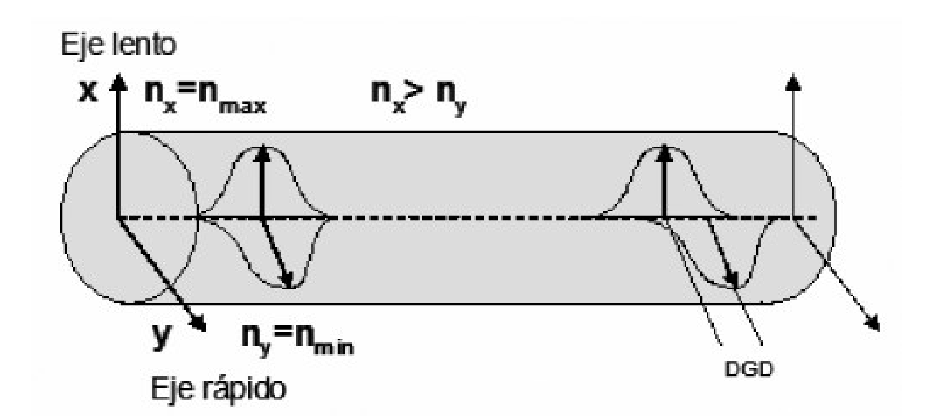
\includegraphics[width=\textwidth]{img/P5_1.png}
		\caption{Se tiene un esquema de la propagacion de dos modos de polarizacion en una fibra optica. donde se ve que no esta presente el efecto de la birrefringencia, es deicr que los modos no se desfasan en sus polaridades}
		\label{fig:first}
	\end{subfigure}
	\hfill
	\begin{subfigure}{0.4\textwidth}
		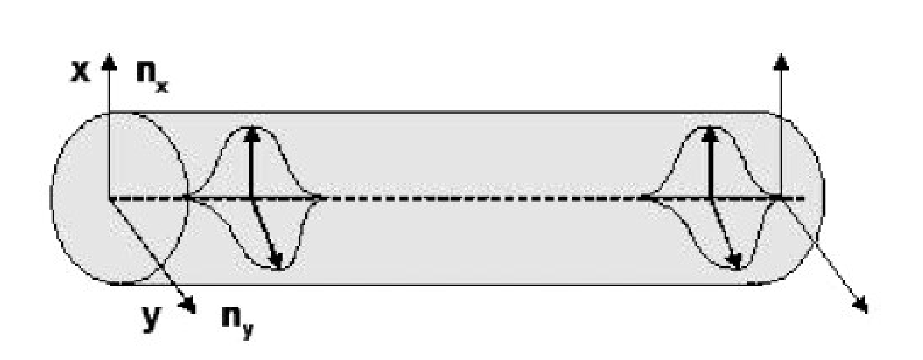
\includegraphics[width=\textwidth]{img/P5_2.png}
		\caption{Se tiene un esquema de la propagacion de dos modos de polarizacion en una fibra optica. donde se ve que esta presente el efecto de la birrefringencia, es deicr que los modos se se desfasan en sus polaridades con un cierto DGD}
		\label{fig:second}
	\end{subfigure}
	\hfill
	\begin{subfigure}{0.4\textwidth}
		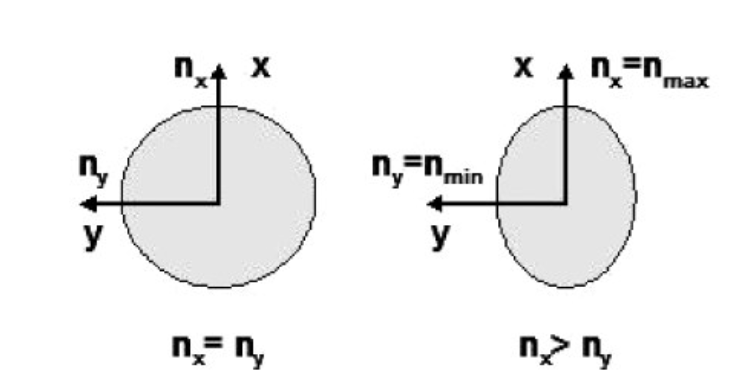
\includegraphics[width=\textwidth]{img/P5_3.png}
		\caption{Corte transversal del nucleo de la fibra optica, donde en el primero no se produce el efecto de birrefringencia y en el segundo si se produce. esto debido al proceso de fabricacion que se menciono con anterioridad}
		\label{fig:third}
	\end{subfigure}
			
	\caption{Esquema obtenido del documento entregado, que nos permite visualizar el efecto de La birrefringencia en la fibra optica.}
	\label{fig:figures}
	\end{figure}
\item \textbf{Los investigadores le consultan si para el sistema óptico bosquejado en el punto
3 se podría tener una fibra óptica de alta eficiencia que compense la dispersión cromática
usando redes de difracción de Bragg en la fibra}\\\\
Se busca el argumentar porque puede ser util el utilizar redes de difraccion de Bragg en la fibra optica para compensar la dispersion cromatica, es por esto que tenemos que definir y comprender previamente ciertos conceptos:
\begin{itemize}
	\item \textbf{Dispersion cromatica:} Es un fenómeno que ocurre cuando diferentes longitudes de onda de la luz viajan a distintas velocidades a través de un medio, como una fibra óptica. Esto sucede porque el índice de refracción del material varía en función de la longitud de onda, lo que provoca que los pulsos de luz se ensanchen a medida que se propagan.
	\begin{figure}
		\centering
		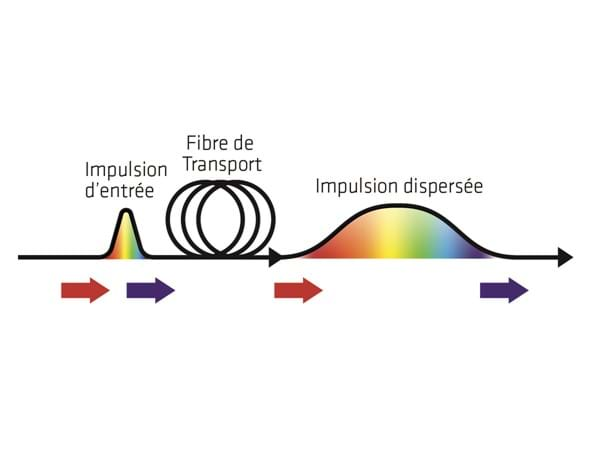
\includegraphics[width=0.5\linewidth]{img/P6_1.jpg}
		\caption{visualizacion de la dispersion cromatica, donde se observa como el pulso se ensancha a medida que se propaga debido a la diferentes velocidades de propagacion de los distintos colores de la luz}
		\label{fig:imagen1}
	\end{figure}
	\item \textbf{Fibras FBG:} Son dispositivos ópticos que se utilizan para filtrar y reflejar ciertas longitudes de onda de la luz. Están hechos de una fibra óptica que ha sido modificada para tener un índice de refracción periódico a lo largo de su longitud. Esto crea una rejilla de difracción que refleja ciertas longitudes de onda de la luz y permite que otras pasen a través de la fibra. Esto esta determinado por:
	\begin{align}
		\lambda = 2n\Lambda
	\end{align}
	Donde $\lambda$ es la longitud de onda Bragg reflejada, n es el indice de refraccion de la fibra y $\Lambda$ es el periodo de la rejilla de difraccion. Esto se logra visualizar como:
	\begin{figure}
		\centering
		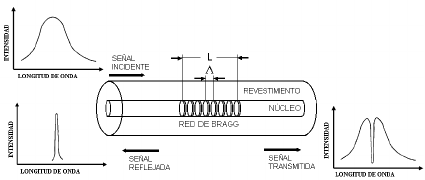
\includegraphics[width=0.6\linewidth]{img/P6_2.png}
		\caption{visualizacion de una fibra FBG, donde se observa la rejilla de difraccion que refleja ciertas longitudes de onda de la luz y permite que otras pasen a traves de la fibra}
		\label{fig:imagen2}
	\end{figure}
	Esto tiene variadas aplicacione pero principalmente para la compensacion de la dispersion cromatica en las fibras opticas, ya que permite reflejar ciertas longitudes de onda y permitir que otras pasen a traves de la fibra, esto se logra mediante el siguiente esquema:
	\begin{figure}
		\centering
		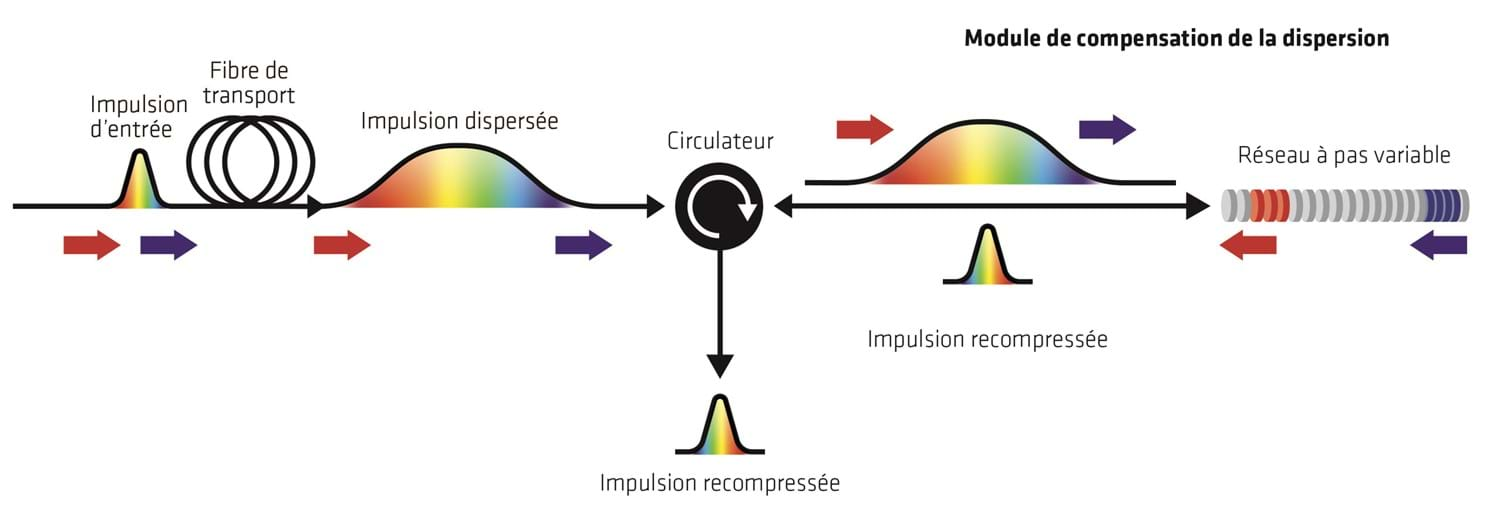
\includegraphics[width=0.7\linewidth]{img/P6_3.jpg}
		\caption{visualizacion de la compensacion de la dispersion cromatica mediante una fibra FBG, donde se observa como la fibra refleja ciertas longitudes de onda y permite que otras pasen a traves de la fibra}
		\label{fig:imagen3}
	\end{figure}
	\item \textbf{Fibras CFBG:} Las fibras de rejilla de Bragg con chirp (CFBG) son una variación de las FBG, pero con la característica de que el espaciamiento entre las rejillas no es constante, sino que varía a lo largo de la fibra. Esto permite que las CFBG reflejen diferentes longitudes de onda a lo largo de la fibra, lo que permite poder compensar en un rango de longitudes de onda mas amplio. Esto se logra visualizar como:
	\begin{figure}
		\centering
		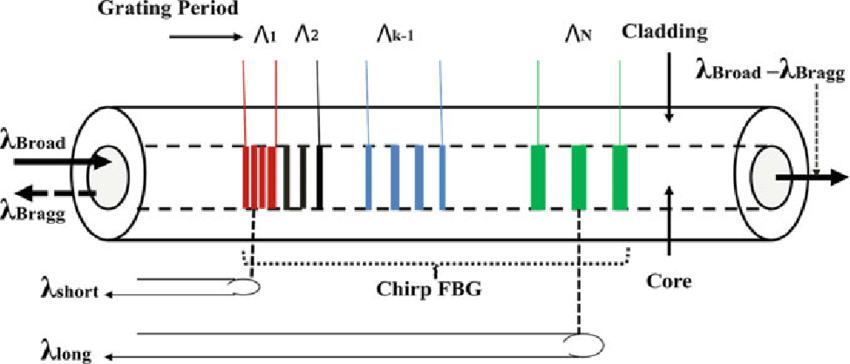
\includegraphics[width=0.6\linewidth]{img/P6_5.png}
		\caption{visualizacion de una fibra CFBG, donde se observa la rejilla de difraccion que refleja diferentes longitudes de onda a lo largo de la fibra}
		\label{fig:imagen4}
	\end{figure}
	Con lo que finalmente podemos concluir que CPFG es una herramienta util para la compensacion de la dispersion cromatica en las fibras opticas, ya que permiten reflejar ciertas longitudes de onda y permitir que otras pasen a traves de la fibra, lo que permite compensar la dispersion cromatica y mejorar la calidad de la transmision de datos.
\end{itemize}
\item Utilizando el Simulador OptiSystem diseñe un sistema óptico a presentar a cliente
considerando los parámetros ópticos del punto 3. 
\begin{itemize}
	\item \textbf{Captura de Pantalla de Diseño óptico global que cumple lo solicitado en el punto
	3 y capturas de pantalla de los parámetros configurados por cada componente y
	visualizaciones de potencias ópticas y pérdidas del sistema.}
	Se busca el realizar un diseño optico en base a los parametros entregados en el punto 3, para ello se tiene que los parametros corresponden a:
	\begin{table}[ht]
		\centering
		\begin{tabular}{|c|c|}
		\hline
		\textbf{Característica}             & \textbf{Valor} \\ \hline
		Sensibilidad óptica                 & -25 dBm        \\ \hline
		Potencia de saturación              & -9 dBm         \\ \hline
		Margen de seguridad                 & 1 dB           \\ \hline
		Pérdida por conectores              & 0,5 dB         \\ \hline
		Carretes de FO                      & 10 km          \\ \hline
		Pérdida por empalmes                & 0,03 dB        \\ \hline
		Atenuación de la fibra              & 0,2 dB/km      \\ \hline
		Potencia Salida transmision             & -17 dBm/km      \\ \hline
		\end{tabular}
		\caption{Características de los equipos ópticos}
		\label{tab:caracteristicas_opticas}
		\end{table}
		Luego mediante el simulador \textit{OptiSystem} se realiza el esquema en donde se consideran todos estos aspectos, el esquema general se visualiza en :
		\begin{figure}
			\centering
			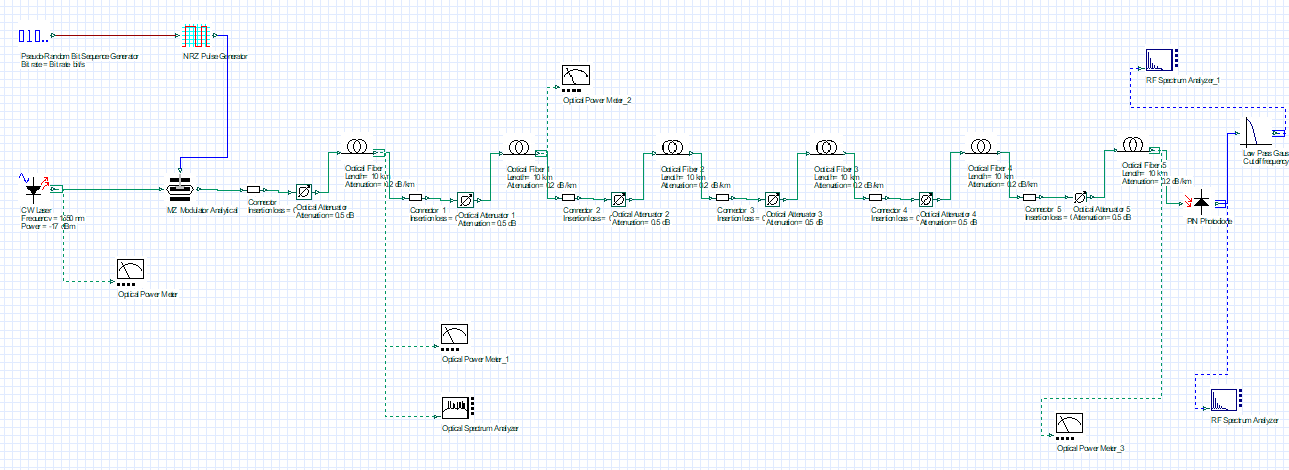
\includegraphics[width=0.9\linewidth]{img/P7_1.png}
			\caption{Esquema general del diseño optico realizado en OptiSyste, donde se subdivide la fibra optica, considerando el largo de 10km ademas de que se adicionan las perdidas por empalme, atenuacion de la fibra y perdida por conectores}
			\label{fig:imagen1}
		\end{figure}
		Luego para el analisis de frecuencias tenemos lo siguiente:
		\begin{figure}
			\centering
			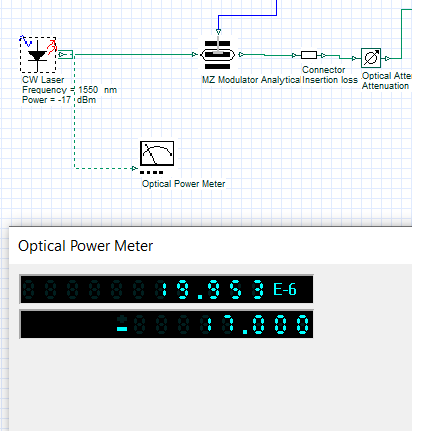
\includegraphics[width=0.4\linewidth]{img/P7_2.png}
			\caption{Potencia de salida del transmisor, la cual corresponde a los -17 dBm esperados.}
			\label{fig:imagen1}
		\end{figure}
		Por otro lado tenemos que la potencia de llegada viene dada por:
		\begin{figure}
			\centering
			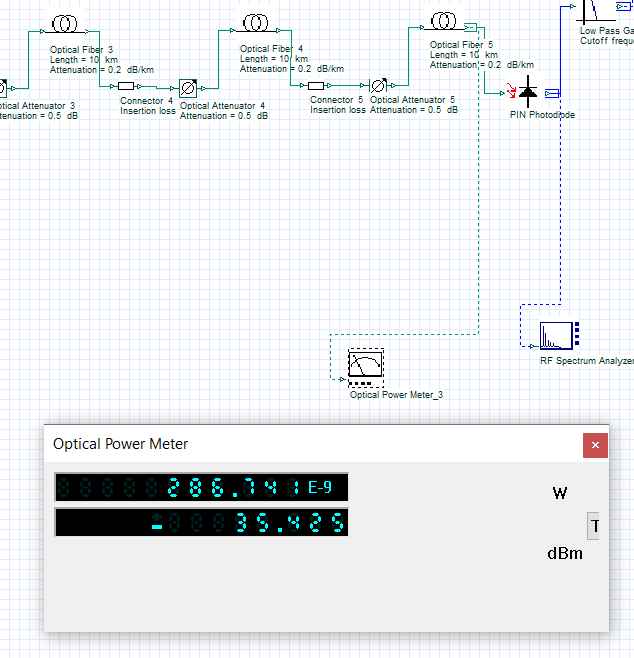
\includegraphics[width=0.4\linewidth]{img/P7_3.png}
			\caption{Potencia de llegada al receptor, la cual corresponde a -35.425 dBm}
			\label{fig:imagen1}
		\end{figure}
		Con lo que podemos corroborar que existen perdidas debidos a los diferentes perdidas asociadas al sistema. Esta potencia se puede obtener de manera teorica como:
		\begin{itemize}
			\item \textbf{Datos importantes:}
			\begin{itemize}
				\item Distancia: 60 km.
				\item Atenuación de la fibra: 0,2 dB/km.
				\item Pérdida por conectores: 0,5 dB por conector (6 conectores).
				\item Pérdida por empalmes: 0,03 dB por empalme (6 empalmes).
				\item Margen de seguridad: 1 dB.
				\item Potencia de salida promedio: (-25 dBm + -9 dBm) / 2 = -17 dBm.
			\end{itemize}
			
			\item \textbf{Cálculos:}
			\begin{itemize}
				\item Atenuación total por la fibra: \( 0,2 \, \text{dB/km} \times 60 \, \text{km} = 12 \, \text{dB} \).
				\item Pérdida por conectores (6 conectores): \( 0,5 \, \text{dB} \times 6 = 3 \, \text{dB} \).
				\item Pérdida por empalmes (6 empalmes): \( 0,03 \, \text{dB} \times 6 = 0,18 \, \text{dB} \).
				\item Pérdidas totales (incluyendo margen de seguridad): \( 12 \, \text{dB} + 3 \, \text{dB} + 0,18 \, \text{dB} + 1 \, \text{dB} = 16,18 \, \text{dB} \).
			\end{itemize}
			
			\item \textbf{Potencia de llegada teórica:} 
			\begin{itemize}
				\item Potencia de salida - pérdidas totales = \( -17 \, \text{dBm} - 16,18 \, \text{dB} = -33,18 \, \text{dBm} \).
			\end{itemize}
		\end{itemize}
		Se observa que el valor difere en 2.245 dBm, esto puede deberse a aspectos de simulacion, pero se aproxima bastante a lo esperado de manera teorica.
	\item \textbf{Cree un nuevo Diseño óptico basado en el inicial utilizando y aprovechando al máximo la aplicación OptiSystem, cambiando o agregando componentes, y/o mejorando los parámetros si es necesario para mostrar un segundo diseño a los ingenieros de ESO
	ampliando la distancia a 130Km para llegar al centro de Antofagasta. ¿Será posible?}\\\\
	Dado que se quiere diseñar un nuevo sistema optico para llegar al centro de Antofagasta, se tiene que considerar que la distancia es de 130 km, se tiene el siguiente sistema extrapolado de lo visto con anterioridad (Es decir, sin implementar alguna tecnica de compensacion)
	\begin{figure}
		\centering
		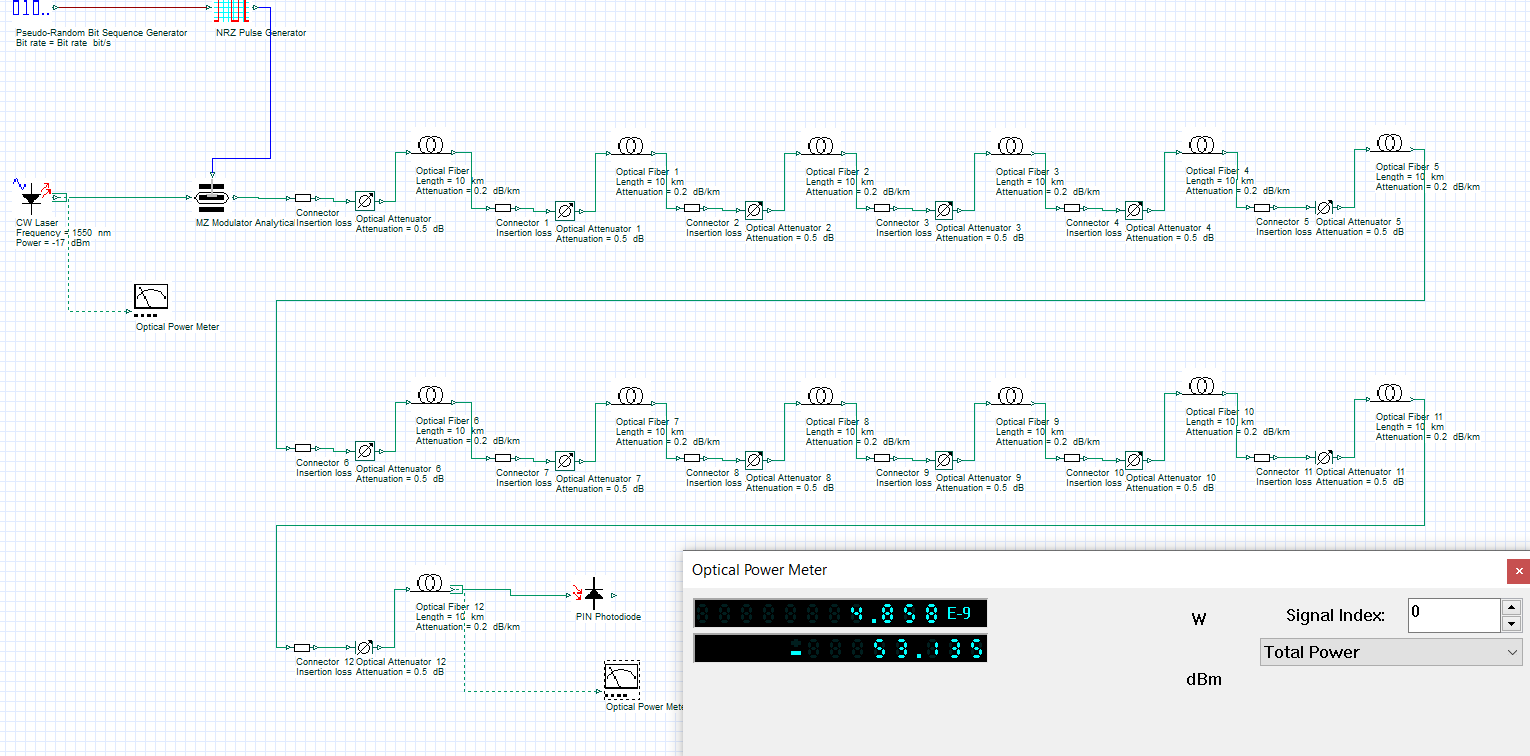
\includegraphics[width=0.9\linewidth]{img/P7_4.png}
		\caption{Esquema general del diseño optico realizado en \textit{OptiSystem}, donde se subdivide la fibra optica, considerando el largo de 130km ademas de que se adicionan las perdidas por empalme, atenuacion de la fibra y perdida por conectores, esto sin considerar alguna modificacion}
		\label{fig:imagen1}
	\end{figure}
	Se observa que se obtiene una potencia de llegada de -53.125 dbM, lo cual es bastante baja y podria tener variadas complicaciones para el proposito de la ESO. Una de las variadas opciones que pueden solucionar este problema corresponde a:
	\begin{itemize}
		\item Aumentar la potencia de salida del transmisor
		\item Utilizar amplificadores ópticos para aumentar la potencia de la señal
		\item Reducir las perdidas , tratando de utilizar carretes de FO mas largos.
	\end{itemize}
	Teniendo en consideracion estos aspectos anteriormente mencionados, tenemos el siguiente esquema
	\begin{figure}
		\centering
		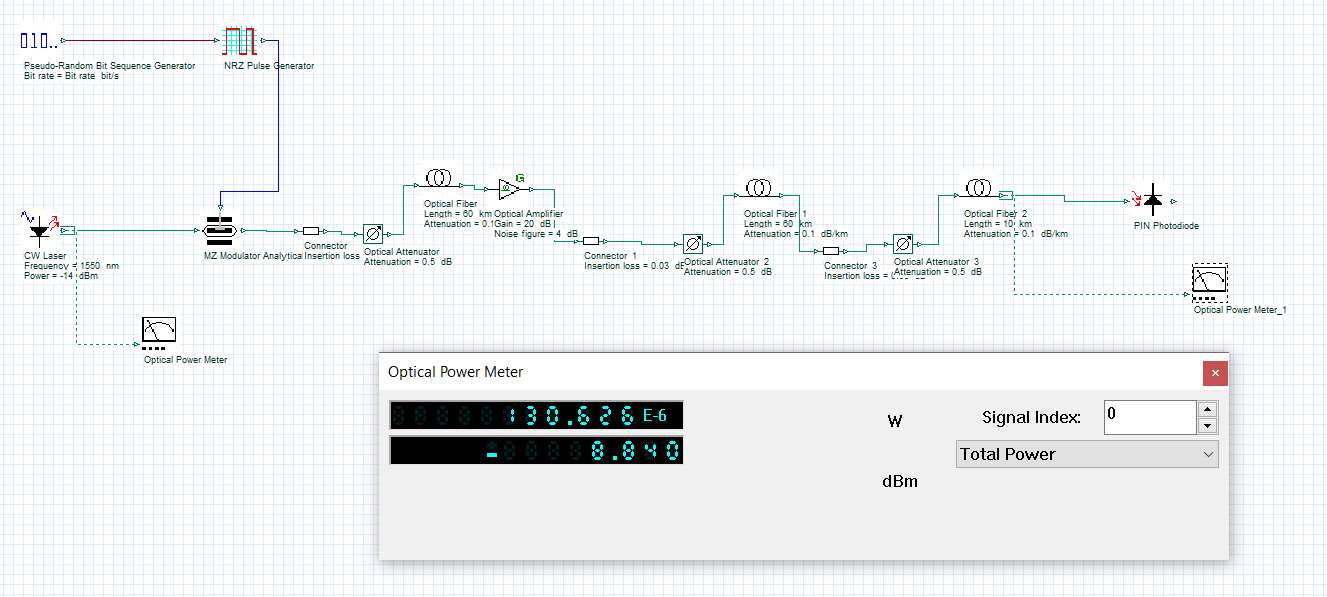
\includegraphics[width=0.9\linewidth]{img/P7_5.png}
		\caption{Esquema general del diseño optico realizado en \textit{OptiSystem}, en la cual se consideran aspectos de mejora de la señal permitiendo que el sistema pueda operar en 130Km con una potencia de llegada aceptable}
		\label{fig:imagen1}
	\end{figure}
	Luego se cosnideran los siguientes aspectos:
	\begin{itemize}
		\item La potencia de salida pasa de -17dbm a -14dbm
		\item Se utiliza un amplificador de 20dB en el Luego del primer carril de FO
		\item Se reduce la cantidad de empalmes y conectores haciendo que los carriles de fibra optica sea de 60Km en vez de los 10km que teniamos antes 
		\item Se reducen las atenuaciones de la fibra optica a 0.1dB por kilometro solamente.
	\end{itemize}
	Teniendo en cuenta todo lo anterior se logra un muy buen resultado a la salida de la fibra optica, con una potencia de -8.840 dbm, lo cual es un valor aceptable para la transmision de datos.
\end{itemize}

\end{enumerate}